\chapter{Manuales}


\section{Manual de usuario}
\bigskip





\section{Manual de despliegue}
\bigskip

A continuación se explicará la forma y requisitos de despliegue del sistema. 

\subsection{Requisitos para el despliegue}
\bigskip

Para el correcto despliegue de la aplicación habrá que contar con sus 2 partes: el servicio web y el procesamiento con GPU mediante CUDA.

\bigskip
Para lanzar el servicio web:
\begin{itemize}
	\item Apache (versión 2.4 o superior)
	\item Python (Python 2)
	\item Django  (versión 1.10 o superior)
\end{itemize} 

\bigskip
Y para el procesamiento mediante CUDA:
\begin{itemize}
	\item Dispositivo NVIDIA
	\item Drivers NVIDIA (versión 352.xx)
	\item CUDA 7.5
	\item C++ (versión 4.x)
\end{itemize} 

\subsection{Despliegue}
\bigskip


Una vez que se cumplen los requisitos, sólo habrá que lanzar el servicio web, ya que el procesamiento usando la GPU se gestiona sólo mediante el ejecutable \textit{geneticAlgorithm}.

Para ello el servidor Apache tendrá que estar activo (se puede activar ejecutando \textit{service apache2 restart}) y lanzar el proyecto Django con el proyecto: dentro del directorio SWGPU ejecutar, junto con la URL donde lanzar el sistema \textit{python manage.py runserver [URL]}


\subsection{Despliegue automatizado}
\bigskip
También se proporcionará el script o archivo \textit{despliegue.sh} para automatizar la tarea de despliegue.

Simplemente habrá que ejecutarlo (dentro del \textit{directorio SWGPU},mediante la orden \textbf{sudo ./despliegue.sh}) y luego especificar la URL donde se desplegará. El script comprobará los requisitos antes citados, preparará el servidor y lanzará el sistema.

En la siguiente captura se ve como se lanza el servidor:

\bigskip
\begin{figure}[h]
	\centering
	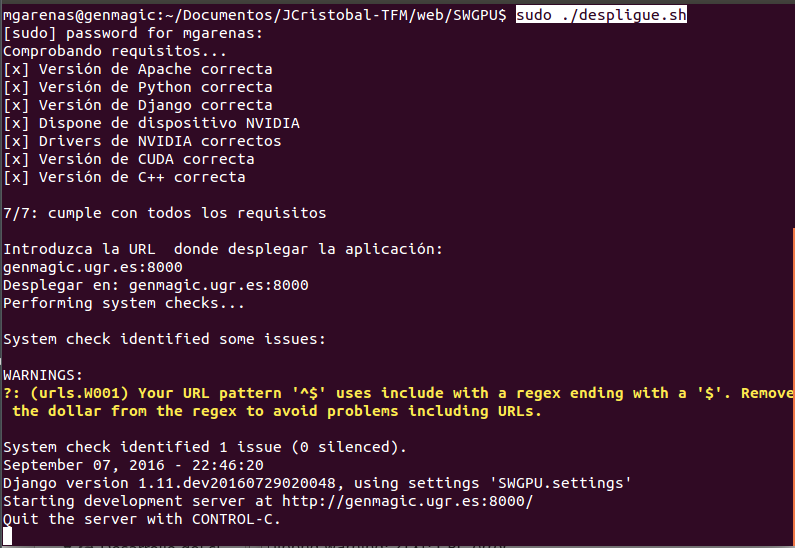
\includegraphics[width=1\linewidth]{../images/prueba_despliegue}
	\caption[Captura del despliegue automático]{Captura del despliegue automático}
	\label{fig:prueba_despliegue}
\end{figure}


